\documentclass[oneside]{article}
\usepackage[utf8]{inputenc}
\usepackage{mathtools}
\usepackage{graphicx}
\usepackage{hyperref}


\title{AerE 161 \\ Project \#2: Flight Path of a Projectile}
\author{Hammad Imam \\ Undergraduate, Aerospace Engineering \\ Iowa State University}
\date{March 23rd,	2018}

\begin{document}

\begin{titlepage}
\maketitle
\end{titlepage}

\clearpage
\tableofcontents

\newpage

\section{Problem Statement}
The purpose of this assignment was to study the effects of air resistance on the flight path of projectiles. Since objects behave differently with and without air resistance, two formulas were used to calculate trajectories. This project utilizes 5 different .m files to calculate the data, plot different graphs, and to pass values to be calculated and plotted. As the output, 6 graphs were generated.

\newpage
\section{Theory}
\subsection{Introduction and Symbols Used}
In this section, the methods of calculation for the graphs will be discussed. The first step will be explaining the approach taken to calculate the values. After that, the equations will be given and the reasoning behind them will be explained, first for projectiles without air resistance, then for projectiles with air resistance. All calculations used in the code will be explained in this section.

The following symbols will be used in this section
\begin{itemize}
    \item $t$ - time, [s]
    \item $k$ - Coefficient of Resistance, [1/s]
    \item $x$ - Horizontal Position or Distance, [m]
    \item $y$ - Vertical Position or Altitude, [m]
    \item $v_0$ - Launch velocity, [m/s]
    \begin{itemize}
        \item $v_{0x}$ - x component of launch velocity, [m/s]
        \item $v_{0y}$ - y component of launch velocity, [m/s]
    \end{itemize}
    \item $\theta$ - Launch angle from the horizontal, [deg]
\end{itemize}
\subsection{Approach}
When finding the trajectory, both position and velocity in the x and y directions need to be calculated. All of these can be found as functions of time, so the first step in generating these values will be to find the time that the object spends travelling. After the time it takes to travel the whole distance is found, the time can be stepped up from 0 to its maximum value and the kinematic equations can be found in terms of time, $t$. These can all be incorporated into vectors such that the nth element of any vector corresponds to the value of that vector at the time at the nth element of the time vector. All of these vectors will be incorporated into a struct for a single value of the air resistance coefficient, $k$. These structs will then be combined into a single struct array containing all kinematic values for the given values of $k$.

\subsection{Finding Total Time Elapsed}
An object is "in the air" from when it leaves the ground to when it returns, so it follows that the total time elapsed will be at the instant that the object hits the ground. In more algebraic terms, if $y(t)$ is the height of the object as a function of time, then $y(t_\textrm{max}) = 0$. To find this, we will use the equation for $y$, set it equal to 0, and solve for $t$.

\begin{align*}
    y(t) = v_0sin(\theta)t - \frac{1}{2}gt^2\\
    0 = t(v_0sin(\theta) - \frac{g}{2}t)\\
    t = 0, t = \frac{2v_0sin(\theta)}{g}
\end{align*}

Solving for $t$ gives us two values. However, the first one is 0, and since we're launching at $t=0$, we already know that that point gives us $y=0$. The second point is the one we're more interested in. This gives us the equation for time elapsed from launch to landing, so our equation for time elapsed is 

\begin{align}
    t = \frac{2v_0sin(\theta)}{g}
\end{align}

The issue now comes up that this $t$ value is calculated using the $y$ equation without air resistance being taken into account. Since the air resistance prevents the object from gaining as much speed as it would without air resistance, we can safely make the assumption that the time elapsed with air resistance will be the same or lower than the time elapsed without. In the code, since we are stepping the $t$ value up and calculating values based on that, we can cover all cases by stopping to step $t$ up either at the calculated value for $t_{max}$ or as soon as the calculated value for $y$ is equal to 0. 

Since the $t$ portion of the calculation is taken care of, the equations for the  kinematic components can be listed and we can begin to use them in the calculations.

\subsection{Without Air Resistance ($k = 0$)}
\subsubsection{Horizontal Velocity, $v_x$, m/s}
\begin{align}
    v_x(t) = v_0cos(\theta)
\end{align}
\subsubsection{Vertical Velocity, $v_y$, m/s}
\begin{align}
    v_y(t) = v_0sin(\theta) - gt
\end{align}
\subsubsection{Distance, $x$, m}
\begin{align}
    x(t) = v_0cos(\theta)t
\end{align}
\subsubsection{Altitude, $y$, m}
\begin{align}
    y(t) = v_0sin(\theta)t - \frac{1}{2}gt^2
\end{align}

\subsection{With Air Resistance ($k \neq 0$)}
\subsubsection{Horizontal Velocity, $v_x$, m/s}
    \begin{align}
        v_x(t) = v_0cos(\theta)e^{-kt}
    \end{align}
\subsubsection{Vertical Velocity, $v_y$, m/s}
    \begin{align}
        v_y(t) = v_0sin(\theta)e^{-kt} + \frac{g}{k}(e^{-kt} -1)
    \end{align}
\subsubsection{Distance, $x$, m}
    \begin{align}
        x(t) = \frac{v_0cos(\theta)}{k}(1-e^{-kt}
    \end{align}
\subsubsection{Altitude, $y$, m}
    \begin{align}
        y(t) = -\frac{gt}{k} + \frac{kv_0sin(\theta) + g}{k^2}(1-e^{-kt})
    \end{align}
\subsection{Conclusion}
Now that we have all our equations, it's time to make sure that we have all our variables in order to calculate what we need. $g$ is a known constant, $v_0$ and $\theta$ will be given in the problem, and $t$ and $k$ will be produced by the code. Since we have everything we need, it's safe to move forwards and use the code to generate results.\\

\clearpage

\section{Solution}
\subsection{Overview}
This section contains the solution to the problem, which is 5 .m files and 6 graphs. The .m files all contain comments at the start that describe the purpose of that file, and then more comments in the body that describe what the code is doing. 
\subsection{Code}
\subsubsection{flightpath.m}
This is the main function that provides the data used for other .m files. It receives values for $v_0$, $\theta$, $k$. The data is provided in a 1$\times$n struct where n is the length of the k value that is passed to it. Each element of the struct contains vectors for $t$, $v_x$, $v_y$, $x$, and $y$.\\ 
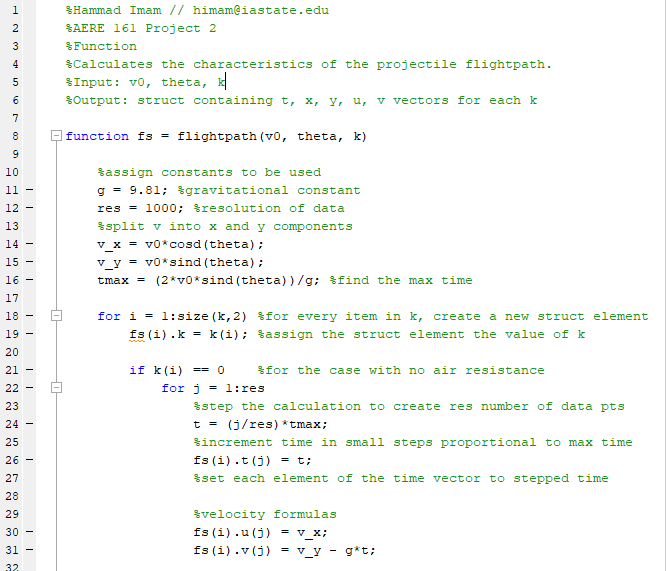
\includegraphics [width=\linewidth]{code_flightpath1.png}
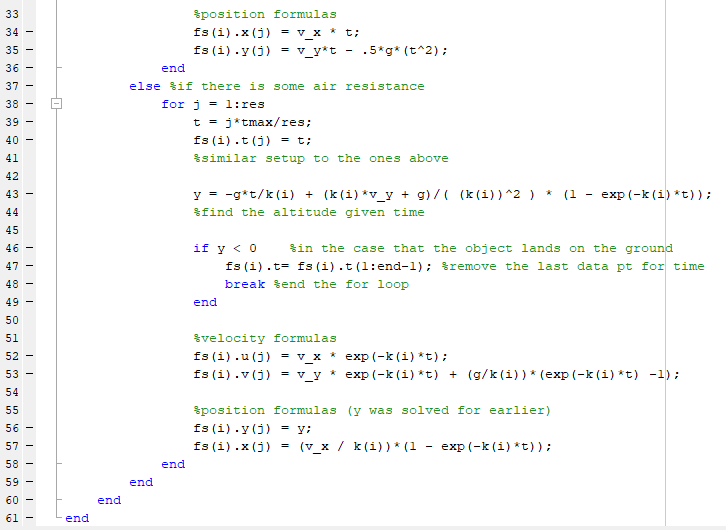
\includegraphics [width=\linewidth]{code_flightpath2.png}
\subsubsection{plot\_flightpaths.m}
This is a function that takes the struct generated by flightpath.m and outputs 4 graphs: $y(x)$, $y(t)$, $v_x(t)$, and $v_y(t)$.\\
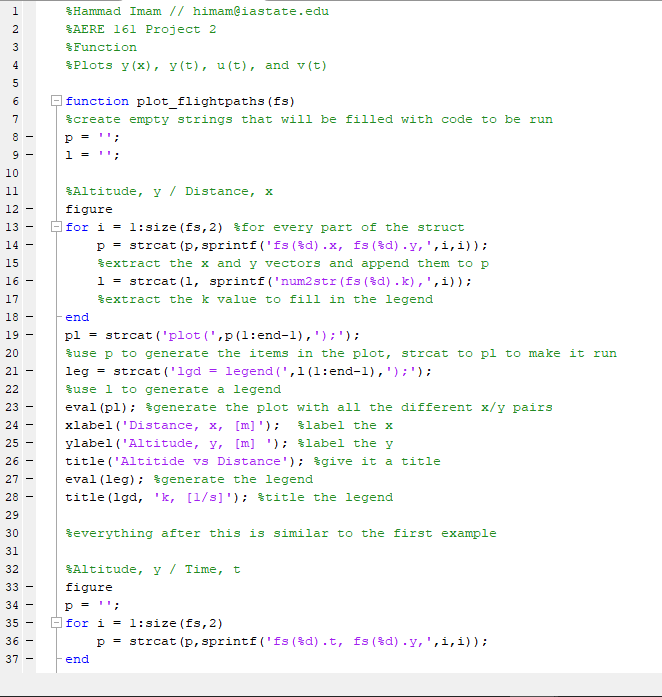
\includegraphics [width=\linewidth]{code_plot_flightpaths1.png}
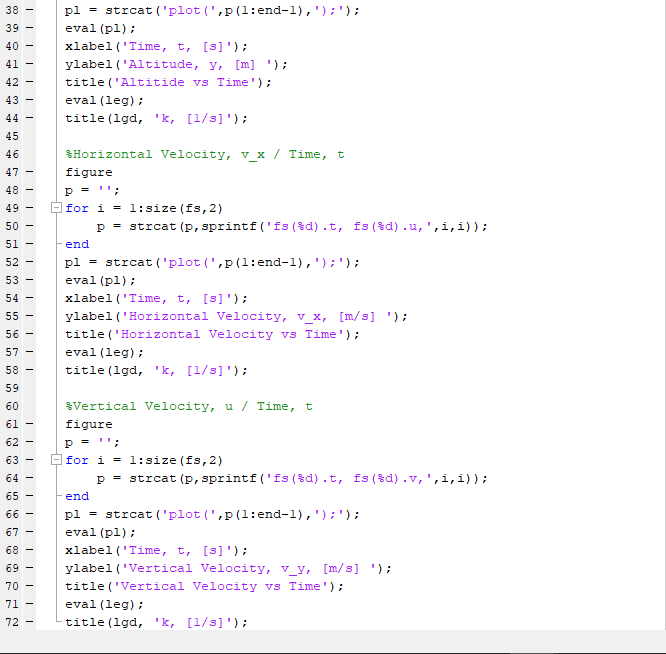
\includegraphics [width=\linewidth]{code_plot_flightpaths2.png}
\subsubsection{main\_flightpaths.m}
This is a script that gives initial values to flightpath.m, receives that data, and passes it to plot\_flightpaths.m to output graphs.\\
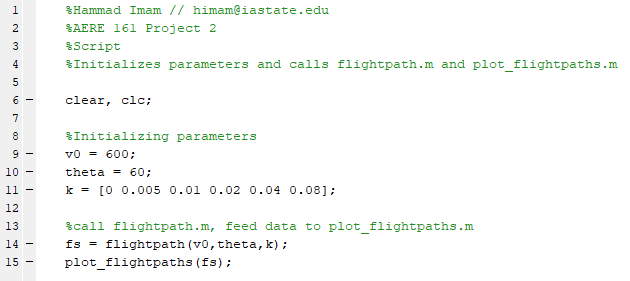
\includegraphics [width=\linewidth]{code_main_flightpaths.png}
\subsubsection{plot\_range.m}
This is a function that takes the struct generated by flightpath.m and outputs 2 graphs: $x(k)$, $t_{max}(k)$.\\
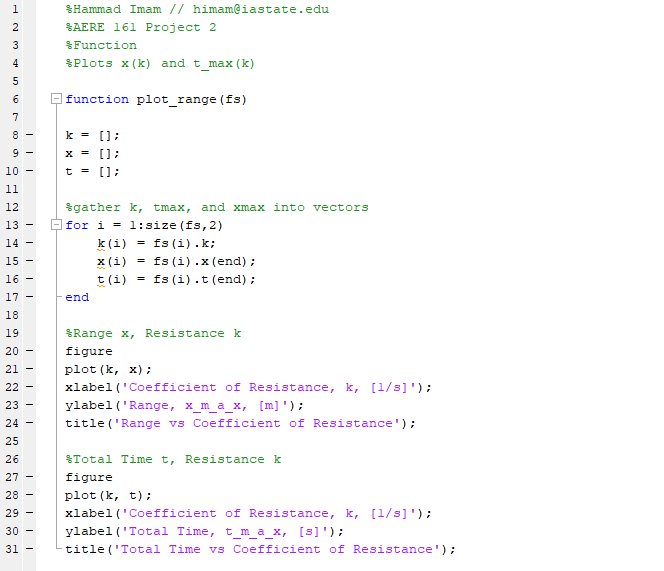
\includegraphics [width=\linewidth]{code_plot_range.png}
\subsubsection{main\_range.m}
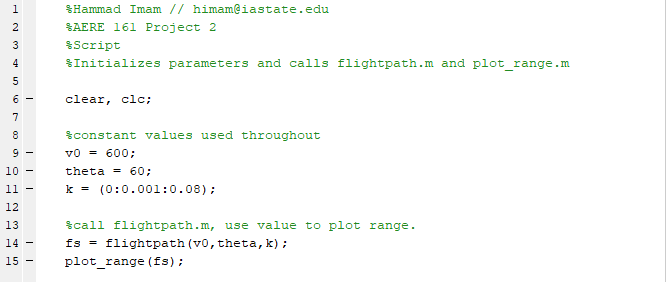
\includegraphics [width=\linewidth]{code_main_range.png}
\newpage
\subsection{Plots}
\subsubsection{Altitude y vs. Distance x}
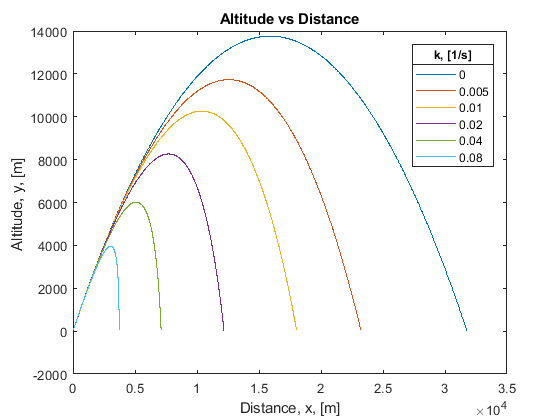
\includegraphics [width=\linewidth]{graph_y-x.png}
\subsubsection{Altitude y vs. Time t}
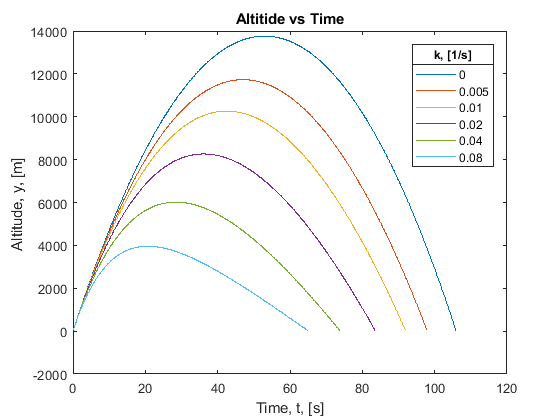
\includegraphics [width=\linewidth]{graph_y-t.png}
\subsubsection{Horizontal Velocity v\_x vs. Time t}
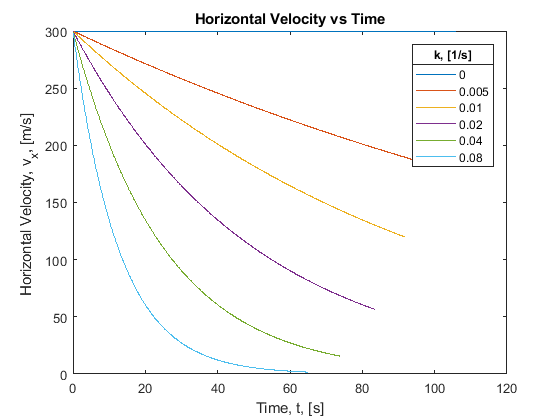
\includegraphics [width=\linewidth]{graph_u-t.png}
\subsubsection{Vertical Velocity v\_y vs. Time t}
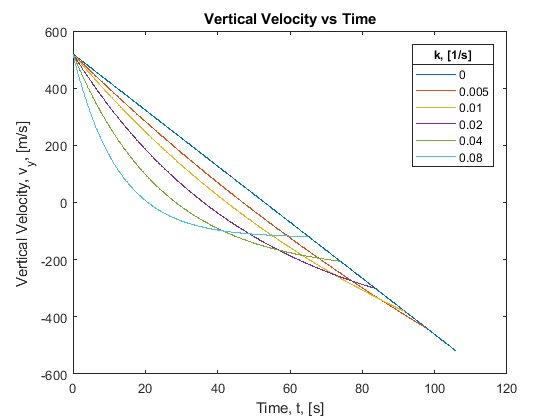
\includegraphics [width=\linewidth]{graph_v-t.png}
\subsubsection{Range x$_max$ vs. Coefficient of Resistance k}
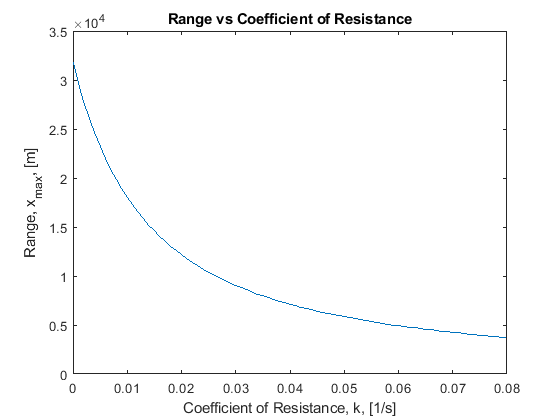
\includegraphics [width=\linewidth]{graph_x-k.png}
\subsubsection{Time t$_max$ vs. Coefficient of Resistance k}
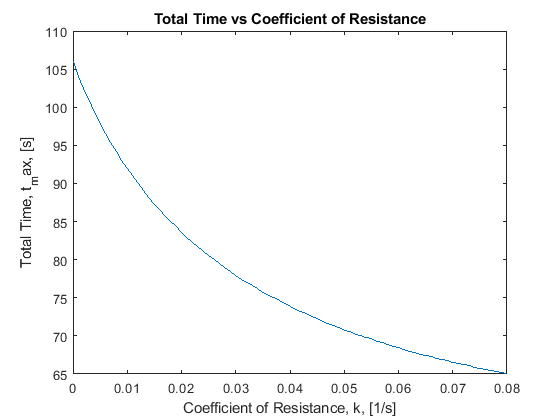
\includegraphics [width=\linewidth]{graph_t-k.png}


\newpage
\section{Discussion}
\subsection{Analysis}
From the graphs produced, we can draw some conclusions about how the projectile behaves. As the coefficient of air resistance increases, both time spent in the air and the range of the projectile decrease, with the range showing a greater decrease. This is because some of the object's kinetic energy is wasted pushing through the air and therefore lost to drag. As a result, the highest altitude reached is also lower. The effects on velocity are interesting, as increasing the coefficient of air resistance causes the vertical velocity to drop faster at the start, but then end along the same line as when there was no air resistance. The horizontal velocity showed that higher k values would lose speed faster, but then hold onto the speed at a more gradual rate, as opposed to the horizontal velocity without any air resistance, which was constant. 
\subsection{Challenges}
My initial approach to this problem was to find the final time and step to that for all values. However, algebraically manipulating the expressions with air resistance proved difficult, so the code was changed to continue advancing until the altitude reached 0. My method of doing this involved using points evenly spaced on some interval, so there was another challenge with finding a number of points that smoothly showed everything, as the resolution required to accurately depict something on some graphs was too low to depict things on other graphs. I ended up playing with the resolution settings and ultimately kept it set pretty high despite the fact that this made generating results take a second or two longer since the calculations became more memory intensive. The biggest problem I had was how to display the data since it needed to be returned as a vector of vectors for every given k value, so I ended up choosing a struct because it was easy for me to mentally associate the k value with the set of vectors. This again caused problems as it quickly became more memory intensive than I had intended, but it worked out fine.
\end{document}
